\documentclass{article}
\usepackage[margin=1in]{geometry}
\usepackage{amsmath,amsthm,amssymb}
\usepackage{bbm,enumerate,mathtools}
\usepackage{tikz,pgfplots}
\usepackage{chessboard}
\usepackage[hidelinks]{hyperref}
\usepackage{multicol} % Problem 35

\newenvironment{question}{\begin{trivlist}\item[\textbf{Question.}]}{\end{trivlist}}
\newenvironment{note}{\begin{trivlist}\item[\textbf{Note.}]}{\end{trivlist}}
\newenvironment{references}{\begin{trivlist}\item[\textbf{References.}]}{\end{trivlist}}
\newenvironment{related}{\begin{trivlist}\item[\textbf{Related.}]\end{trivlist}\begin{enumerate}}{\end{enumerate}}


\begin{document}
  Say that two sequences with distinct elements are in the same equivalence
  class if their first differences have the same signs.
  (e.g. $(1, 3, 2, 3)$ and $(7,8,-1,0)$ are equivalent because their first
  differences are both $(+, -, +)$.)
  \begin{figure}[!h]
    \centering
    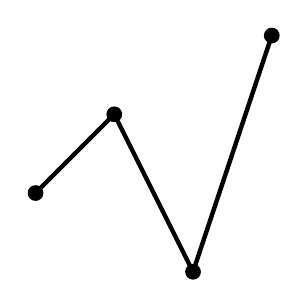
\begin{tikzpicture}
      \draw[ultra thick](0,0)--(1,1)--(2,-1)--(3,2);
      \fill (0,0) circle (0.1cm);
      \fill (1,1) circle (0.1cm);
      \fill (2,-1) circle (0.1cm);
      \fill (3,2) circle (0.1cm);
    \end{tikzpicture}
    \caption{
      $(0, 1, -1, 2)$ has subsequences in the following six equivalence classes:
      $(+, -, +)$, $(+, +)$, $(+, -)$, $(-, +)$, $(+)$, $(-)$. No length $4$
      sequence has its subsequences in more equivalence classes, so $a(4) = 6$.
    }
  \end{figure}

\begin{question}
  What is the general formula for $a(n)$?
\end{question}
\begin{note}
  A quick attempt finds that $a(2) = 1$, $a(3) = 3$, $a(4)=6$, and $a(5)=11$.
\end{note}
\begin{related}
  \item What if the sequences do not necessarily consist of distinct elements?
  \item What if two sequences are considered to be equivalent if they are in the
    same ``sort order''; that is, if both sequences have their biggest element
    in the same position, their second biggest in the same position, and so on.
  \item What if $(+, +) \sim (+)$?
  \item Is the number of equivalence classes for the subsequences determined by
   the number of local minima and maxima?
\end{related}

\end{document}
